\subsection{Prikdosering} \label{Prikplacering}
Der er i den morfologisk analyse fundet frem til, at prikkerne påføres emnet med en mekanisme der doserer en dråbe. Dette sker uden kontakt til emnet, og der vælges at gøre brug af en eksisterende løsning, der implementeres i robotten. Af eksisterende metoder til præcis dosering af dråber er følgende; Piezoelectric Jet Valves (PeJV), Piezoeletric Pump (PeP)) og Thermal InkJet (TIJ) udvalgt. 

%De 3 metoder undersøges, hvorefter en udvælges. 

%Ud fra vurderingen i \ref{Mekanisk system - vurdering} skal der udvikles en løsningen hvor "farven", påføres materialet uden kontakt. Der vil i det følgdene undersøges løsning muligheder, til at opnå prikplacering. Dette vælges som det første, for at lave overslags bergninger på stellets styrke. 


\textbf{Piezoelectric Jet Valves (PeJV)} fungere ved at en piezoelektrisk aktuator, flytter et stempel op og ned. Når stemplet flyttes op, kan væske bevæge sig ind i dyse hovedet. I det stemplet sænkes igen, vil stemplets kontakt med dyse hovedet, gør at væsken skydes ud af dysen, som vist i figur \ref{fig:PeJV}.

\begin{figure}[H]
    \centering
    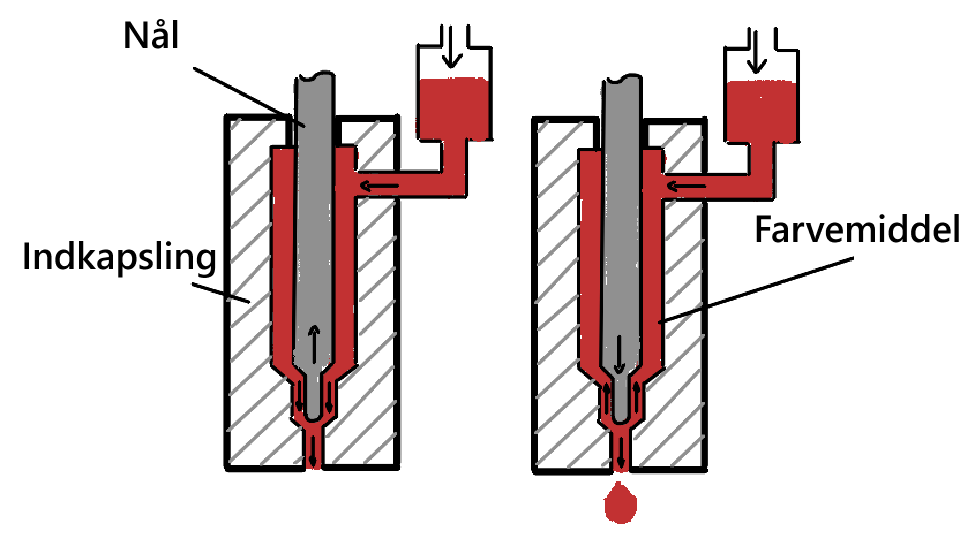
\includegraphics[width=0.6\linewidth]{Sections/5 Konceptgenerering/Media/PEJV.png}
    \caption{Ilustration af piezoelektrisk aktuator}
    \label{fig:PeJV}
\end{figure} \plainbreak{-.5}

 Processen gentages for hver gang der skal sættes en prik. Brugen af piezoelektrisk aktuator, betyder der er en høj kontrol af stemplets bevægelse, hvilket medføre en høj væske doserings præcision, helt ned til \(\SI{0,5}{nL}\). Yderligere betyder brugen af piezoelektrisk aktuator, at cyklussen kan udføres med op til \(\SI{3000}{Hz}\). (\cite{VIEWEG2025JetDV-6210}; \cite{Hoath2016FundamentalsDroplets})


\plainbreak{1}
\textbf{Piezoeletric Pump (PeP)} bruger en piezoelektriske aktuator til at danne et undertryk, som åbner indgangen til et kammer og trækker farve ind i kammeret. Dette fremgår af figur \ref{fig:PeMP}. Når kammeret er fyldt op bruges den piezoelektriske aktuator til at skabe et overtryk, der åbner udgangen og skubber farven ud. Ved PeP skubbes farven ud af et tryk, i modsætning til at blive skudt ud som ved PeJV. Dette resultere i et simplere system, med et begrænset antal dele der bevæges. (\cite{Benaissa2012PerformancesPiezo-pump}; \cite{Hoath2016FundamentalsDroplets})

\begin{figure}[H]
    \centering
    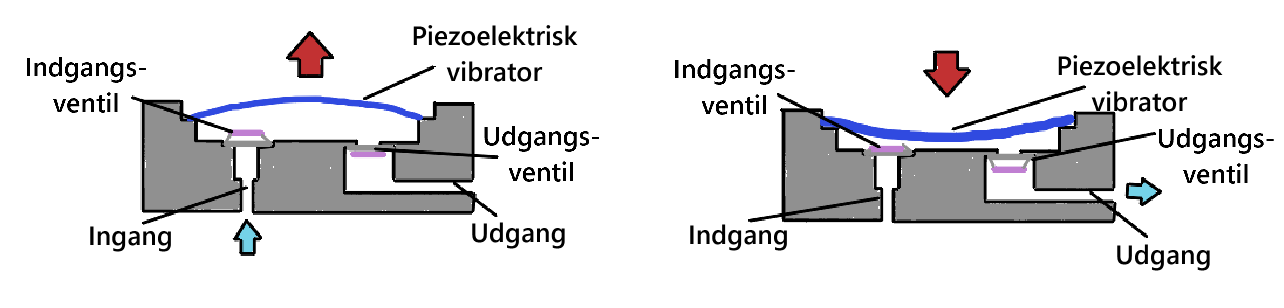
\includegraphics[width=1\linewidth]{Sections/5 Konceptgenerering/Media/pumpe.png}
    \caption{Piezoelektrisk pumpe illustration}
    \label{fig:PeMP}
\end{figure} \plainbreak{-0.5}

PeP bruges ofte til at pumpe en væske kontinuerligt, hvilket betyder der ikke er gode muligheder for udføre doseringer, der kræver pauser imellem. Dette betyder for at gøre brug af PeP, skal der gøres brug af en kontinuerligt væskebevægelse, hvortil et andet system skal opsamle væsken der ikke skal doseres. Sådan et system introducere kompleksitet tilbage i systemet.

\textbf{Thermal InkJet (TIJ)} fungerer ved, at blæk opvarmes indtil det fordamper og der opnås en indre boble i blækket. Den indre boble vil udøve et tryk på blækket, som vil medføre at blækket skubbes ud af en dyse. Når blækket er skubbet tilstrækkeligt ud af dysen, vil boblen kollapse, hvilket resultere i at der skabes et undertryk, der trækker nyt blæk ind til opvarmning, hvorefter processen gentages, dette illustreres på figur \ref{fig:TIJ figur}. \parencite{Hoath2016FundamentalsDroplets}
Ved at gøre brug af opvarmning, har TIJ en begrænsning i forhold til hvor hurtigt der kan printes, da nye bobler først kan dannes efter forrige boble har forladt dysen.


\begin{figure}[H]
    \centering
    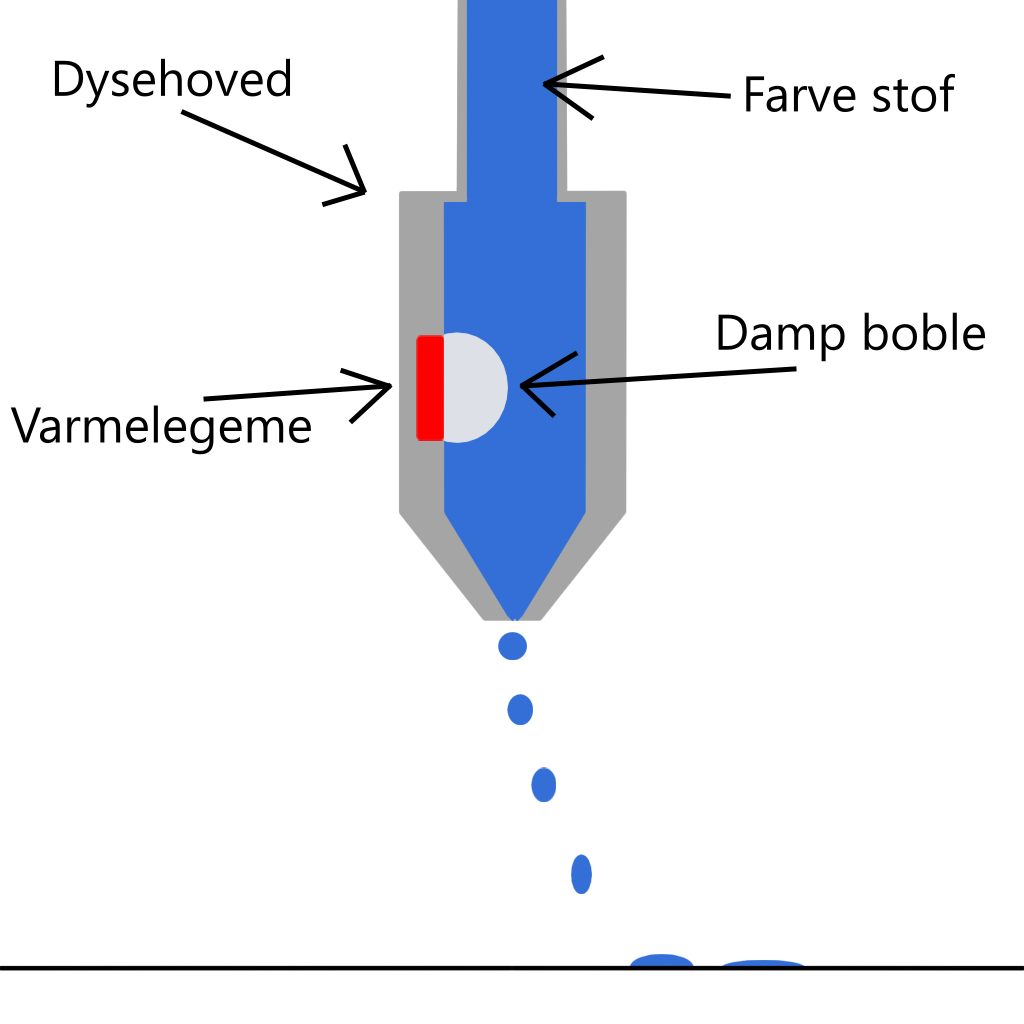
\includegraphics[width=0.3\linewidth]{Sections/6 Detaljeløsning/Media/TIJ figur 2.png}
    \caption{Illustration af thermal injekt teknik.}
    \label{fig:TIJ figur}
\end{figure} \plainbreak{-.5}

\subsubsection{Valg af doserings metode}  \plainbreak{-.5}
Det vælges at der anvendes en PeJV, fordi den kombinerer høj nøjagtighed, med høj gentagelseshastighed (op imod flere tusinde dråber i sekundet) uden at belaste farvestoffet med varme, hvilket sikrer ensartede prikker i den ønskede størrelse. Samtidigt kræver PeJV ikke konstant flow og opsamling af overskydende væske, og den kan producere prikker i et bredt spænd. Alle disse egenskaber understøtter direkte de fremsatte krav omkring nøjagtighed, hastighed og fleksibilitet i speckle-robotten. 
